\documentclass[11pt]{article}
\usepackage[margin=1in]{geometry}
\usepackage{amsmath,amssymb,amsthm,mathtools}
\usepackage{graphicx}
\usepackage{microtype}
\usepackage[hidelinks]{hyperref}
\usepackage{xcolor}

\newtheorem{theorem}{Theorem}
\newtheorem{proposition}{Proposition}
\newtheorem{remark}{Remark}
\DeclareMathOperator{\Op}{Op}
\newcommand{\R}{\mathbb R}
\newcommand{\eps}{\varepsilon}
\newcommand{\ip}[2]{\langle #1,#2\rangle}

\title{A Gaussian Rank-One Obstruction to an\\
Integrable-Spreading Entropy Formula}
\author{Solution packet for arXiv:2603.23744}
\date{11 August 2026}

\begin{document}
\maketitle

\noindent\textbf{Status.}
\texttt{candidate\_counterexample\_likely\_valid}.  This is a full
counterexample to the natural formulation based only on an integrable
spreading function, even with arbitrarily small spreading norm.  It is not a
counterexample to a stricter compact-spreading-support formulation or to a
scaled Szeg\H{o}-limit theorem.

\section{Source question and precise scope}

Allard and B\"olcskei study entropy of compact hypoelliptic
pseudodifferential operators and prove phase-space log-integral asymptotics
under negative-order hypoellipticity and regular variation
\cite{allardbolcskei}.  On printed page 6 they write:
\begin{quote}
``Developing a rigorous analogue of Theorem~1 for underspread operators is an
interesting direction for future work.''
\end{quote}
The preceding sentence anticipates entropy formulae of the same log-integral
form.  The official TeX source's commented development (lines 1078--1098 of
the included \texttt{source\_2603.23744.tex}) makes one contemplated
formulation precise: the spreading function, the symplectic Fourier transform
of the Weyl symbol, has finite $L^1$ norm.

\begin{center}
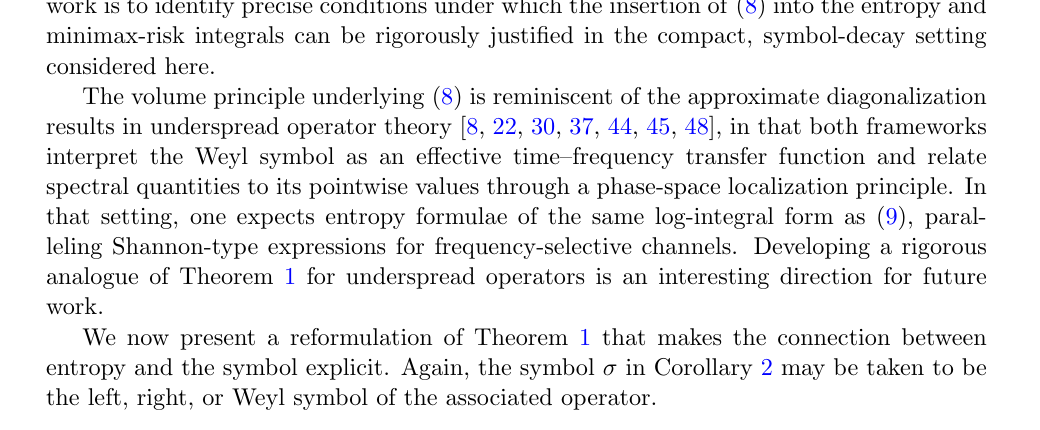
\includegraphics[width=0.94\textwidth]{figures/future_direction_crop.png}
\end{center}

We refute exactly the assertion that this integrable-spreading hypothesis---or
even arbitrary smallness of that norm---is sufficient for
\begin{equation}\label{eq:advertised}
H_T(\eps)\sim
\int_{\R^{2d}}\log_+\!\left(\frac{a(z)}{\eps}\right)\,dz,
\qquad \eps\downarrow0,
\end{equation}
where $a$ is the positive Weyl symbol.  Additional hypotheses can of course
exclude the example; the source paper's own proved theorem does so.

\section{Definitions and idea of the proof}

We use the source's $2\pi$ convention:
\begin{equation}\label{eq:weyl}
(\Op^W(a)f)(x)=\int_{\R^{2d}}
a\!\left(\frac{x+y}{2},\omega\right)
e^{2\pi i(x-y)\cdot\omega}f(y)\,dy\,d\omega.
\end{equation}
For a compact operator on a real Hilbert space, $H_T(\eps)$ is the logarithm
of the least number of closed $\eps$-balls covering $T(B)$.
The spreading function is $\eta=\mathcal F_s a$; the symplectic permutation
does not affect a radial Gaussian or its $L^1$ norm.

\paragraph{Idea of the proof.}
An integrable spreading function controls operator norm, not spectral rank.
A Gaussian rank-one projector has only one entropy axis.  Its strictly
positive Gaussian Weyl symbol, however, exceeds $\eps$ on a $2d$-dimensional
ball of radius comparable to $\sqrt{\log(1/\eps)}$.  Integrating the
logarithmic height over this ball yields order
$(\log(1/\eps))^{d+1}$, whereas the one-axis entropy has order
$\log(1/\eps)$.

\section{Counterexample}

\begin{theorem}\label{thm:main}
For every integer $d\ge1$ and every $\delta>0$, there is a positive,
self-adjoint, rank-one Weyl operator $T$ on real $L^2(\R^d)$ whose Weyl
symbol $a$ is strictly positive and Schwartz, and whose spreading function
$\eta$ is Schwartz with $\|\eta\|_1<\delta$, such that
\[
\frac{H_T(\eps)}{
\displaystyle\int_{\R^{2d}}\log_+(a(z)/\eps)\,dz}
\longrightarrow0.
\]
In particular, \eqref{eq:advertised} fails even at arbitrarily small
spreading $L^1$ norm.
\end{theorem}

\begin{proof}
Let
\[
g(t)=2^{d/4}e^{-\pi|t|^2},\qquad
T_c f=c\,\ip{f}{g}g,
\]
where $c>0$.  Since
$2^{d/2}\int_{\R^d}e^{-2\pi|t|^2}\,dt=1$, the vector $g$ is normalized.
Thus $T_c$ is positive, self-adjoint, and rank one.

Its integral kernel is $K_c(x,y)=cg(x)g(y)$.  Put $u=(x+y)/2$ and
$v=x-y$.  The inverse of \eqref{eq:weyl} at the kernel level gives
\begin{align*}
a_c(u,\omega)
&=\int_{\R^d}K_c(u+v/2,u-v/2)e^{-2\pi i v\cdot\omega}\,dv\\
&=c2^{d/2}e^{-2\pi|u|^2}
  \int_{\R^d}e^{-\pi|v|^2/2}e^{-2\pi i v\cdot\omega}\,dv\\
&=c2^d e^{-2\pi(|u|^2+|\omega|^2)}.
\end{align*}
This is strictly positive and Schwartz.  The $2d$-dimensional Gaussian
Fourier formula, with the harmless symplectic permutation, yields
\begin{equation}\label{eq:eta}
\eta_c(\zeta)=c e^{-\pi|\zeta|^2/2},
\qquad
\|\eta_c\|_1=c2^d.
\end{equation}
Choosing $0<c<\delta/2^d$ proves the asserted arbitrary smallness.

On the real unit ball, $\ip{f}{g}$ ranges over $[-1,1]$, and hence
$T_c(B)=[-c,c]g$.  Projection of any covering center onto the line $\R g$
cannot increase its distance to this interval.  Covering an interval of
length $2c$ by intervals of radius $\eps$ therefore gives, for
$0<\eps<c$,
\begin{equation}\label{eq:entropy}
N(\eps;T_c(B))=\left\lceil\frac c\eps\right\rceil,
\qquad
H_{T_c}(\eps)=\log\left\lceil\frac c\eps\right\rceil
=\log(c/\eps)+o(1).
\end{equation}

It remains to compute the proposed right side.  Set
$L=\log(c2^d/\eps)$ and suppose $0<\eps<c2^d$.  The positive part is
supported on the ball $|z|^2<L/(2\pi)$ in $\R^{2d}$.  If
$v_{2d}=\pi^d/d!$ is its unit-ball volume and
$R^2=L/(2\pi)$, radial integration gives
\begin{align}
I_c(\eps)
&=\int_{|z|<R}(L-2\pi|z|^2)\,dz\notag\\
&=L v_{2d}R^{2d}-2\pi\frac{2d}{2d+2}v_{2d}R^{2d+2}\notag\\
&=\frac{L^{d+1}}{2^d d!(d+1)}.\label{eq:integral}
\end{align}
Equations \eqref{eq:entropy} and \eqref{eq:integral} imply
$H_{T_c}(\eps)/I_c(\eps)\to0$ for every $d\ge1$.
\end{proof}

\section{A separate obstruction to the commented inversion route}

\begin{proposition}\label{prop:bounded}
Suppose an operator has a spreading representation
\[
S=\int_{\R^{2d}}\eta(z)\pi(z)\,dz
\]
in the weak sense, where the time-frequency shifts $\pi(z)$ are unitary and
$\eta\in L^1$.  Then $S$ is bounded and
$\|S\|\le\|\eta\|_1$ (up to the fixed normalization constant of the chosen
spreading convention).  In particular, its eigenvalues cannot tend to
infinity.
\end{proposition}

\begin{proof}
For $f,h\in L^2$, unitarity gives
\[
|\ip{Sf}{h}|
\le\int |\eta(z)|\,|\ip{\pi(z)f}{h}|\,dz
\le\|\eta\|_1\|f\|_2\|h\|_2.
\]
Taking the supremum over unit vectors proves the norm bound.
\end{proof}

The official source comments place finite spreading $L^1$ norm next to an
operator ``whose eigenvalues tend to infinity'' before proposing inversion.
Proposition~\ref{prop:bounded} shows that these conditions cannot describe one
fixed operator under the standard spreading representation.  A coherent
replacement would require a scaling family, another unbounded class, or an
independent spectral-counting hypothesis.

\section{Verification, limitations, and novelty}

The included standard-library script numerically evaluates the radial
integral in 45 combinations of $d,c,$ and $\eps$, checks the arbitrary-norm
scaling in \eqref{eq:eta}, and checks decay of the entropy/integral ratio.  It
returned \texttt{PASS}.  These tests guard arithmetic and normalization; the
proof above is exact and does not depend on computation.

The Gaussian spreading function is not compactly supported.  Therefore the
packet makes no claim against definitions of underspreadness that require
compact spreading support of area below a threshold.  Nor does it contradict
Theorem~1 of the source: $a_c$ is not a negative-order hypoelliptic symbol with
the stated regularly varying volume.  The result instead proves that
integrable spreading alone cannot replace the source theorem's spectral
regularity mechanism.

A bounded novelty search on 11 August 2026 used the exact future-work phrase,
the target title and authors, and combinations of \emph{metric entropy},
\emph{underspread}, \emph{log integral}, \emph{rank one}, and \emph{Wigner}.
It found general approximate-diagonalization and scaled Szeg\H{o}-asymptotic
literature, but no exact Gaussian rank-one entropy obstruction or later answer
to this 2026 direction.  This is not an exhaustive novelty certification.

\paragraph{Human-review recommendation.}
Check first that the source-comment finite-$L^1$ formulation is the intended
scope.  Then verify the Weyl normalization in the kernel calculation and the
compact-support exclusion.  The entropy and radial integration steps are
elementary.

\begin{thebibliography}{9}
\bibitem{allardbolcskei}
T. Allard and H. B\"olcskei,
\emph{Entropy and Minimax Risk of Hypoelliptic Pseudodifferential Operators},
arXiv:2603.23744, 2026.
\end{thebibliography}

\end{document}
